% !TEX root = main.tex
\chapter{Mass fit}
\label{ch:massfit}

\linespread{1.08}\selectfont

After the full selection, the data sample is split into two samples using \dllkpi of the bachelor pion, referred to as \emph{pion} and \emph{kaon} sample:
the \emph{pion} sample has $\dllkpi\leq5.0$ and the \emph{kaon} sample $\dllkpi>5.0$.
This distinction is useful when separating \mbox{\BdToDpi} from $\Bd\!\to\Dm\Kp$ candidates as no dedicated selection cut is needed.
Instead this separation is done statistically in the fit to the invariant mass distribution.

The invariant \Bz mass distributions of candidates with a tag of one of the flavour tagging algorithms are fitted simultaneously in these samples in order to calculate \emph{sWeights}~\cite{Pivk:2004ty}, which are used in the following analysis steps to statistically separate signal from background candidates.
It is important to note that the work described in this chapter was done by a collaborator.
However, since this is an essential part of the analysis required to follow the subsequent steps, it is not omitted completely, but the extent to which \eg experimental techniques are described is less comprehensive compared to the other parts.

When parametrising the invariant \Bz mass, all contributing components need to be described. Backgrounds from semileptonic decays, \mbox{$\Lb\!\to\Lcbar\pip$} decays and \mbox{$\Bs\!\to\Dsm\pip$} decays are either removed in the selection or found to be at a negligible level.
However, beside the signal component and the combinatorial background both, the \emph{pion}- and \emph{kaon} sample show additional backgrounds which arise due to missing neutral particles in the reconstruction or pion-kaon-misidentifications.
In the \emph{pion} sample contributions from $\Bz\!\to\Dm\rhop\!\left(\to\pip\piz\right)$ and $\Bz\!\to\Dstarm\!\left(\to\Dm\piz/\g\right)\pip$ decays arise, the \emph{kaon} sample shows a component from $\Bz\!\to\Dm\Kstarp\!\left(\to\Kp\piz\right)$ and also $\Bz\!\to\Dm\rhop\!\left(\to\pip\piz\right)$ decays which need to be described.
Furthermore, both samples show a cross-feed component from each other.
The number of cross-feed $\Bz\!\to\D\kaon$ candidates in the \emph{pion} sample is expressed from the yield in the \emph{kaon} sample and vice versa as
\begin{equation}
\begin{aligned}
N_{\Bz\!\to\D\pion}^{\kaon}&=\frac{1-\varepsilon_{\text{PID}}\!\left(\Bz\!\to\D \pion\right)_{\pion}}{\varepsilon_{\text{PID}}\!\left(\Bz\!\to\D \pion\right)_{\pion}}\times N_{\Bz\!\to\D\pion}^{\pion} \,\,,\\
N_{\Bz\!\to\D\kaon}^{\pion}&=\frac{1-\varepsilon_{\text{PID}}\!\left(\Bz\!\to\D \kaon\right)_{\kaon}}{\varepsilon_{\text{PID}}\!\left(\Bz\!\to\D \kaon\right)_{\kaon}}\times N_{\Bz\!\to\D\kaon}^{\kaon}\,\,.\label{eq:ConstrainCrossFeed}
\end{aligned}
\end{equation}
Here, the quantities $N_{\Bz\!\to\D X}^{Y}$ ($X,Y=\pion,\kaon$) are the numbers of $\Bz\!\to\D X$ candidates in the $Y$ sample, while $\varepsilon_{\text{PID}}\!\left(\Bz\!\to\D X\right)_Y$ are the corresponding efficiencies of the \dllkpi requirements on simulation.

Before describing the mass fit to data {\cref{sec:MassFitData}}, first the probability density functions (PDFs) used for the different components are introduced in the following.

\section{Probability densitiy functions}
\label{sec:PDFs}

The various peaking components in the invariant mass distributions are described by a phenomenological approach, where the description is first
estimated on simulated decays.
In contrast, the combinatorial background is determined directly in the fit to data.
For the \emph{pion} sample, the following PDFs are used to parameterise the peaking components:
\begin{itemize}
	\item $\Bz\!\to\Dpm\pimp$: The signal component is described by a double-sided Hypatia and a Johnson SU function.
	The Hypatia~\cite{Santos:2013ky} is defined as
	\begin{equation}
	\begin{aligned}
	&\mathcal{I}(m;\mu,\sigma,\lambda,\zeta,\beta,a_1,n_1,a_2,n_2) \propto\\
	&\hspace{2.8cm}\begin{cases}
	G(m,\mu,\sigma,\lambda,\zeta,\beta,a,n), &\,   - a_1 < \frac{m - \mu}{\sigma} < a_2 \\
	\frac{G(\mu - a_1 \sigma,\mu,\sigma,\lambda,\zeta,\beta)}{\left(1 - m/(n \frac{G(\mu - a_1\sigma,\mu,\sigma,\lambda,\zeta,\beta)}{G^\prime(\mu - a_1 \sigma,\mu,\sigma,\lambda,\zeta,\beta)} -a_1 \sigma)\right)^{n_1}},	&\,  - a_1 > \frac{m - \mu}{\sigma} \\
	\frac{G(\mu - a_2 \sigma,\mu,\sigma,\lambda,\zeta,\beta)}{\left(1 - m/(n \frac{G(\mu - a_2\sigma,\mu,\sigma,\lambda,\zeta,\beta)}{G^\prime(\mu - a_2 \sigma,\mu,\sigma,\lambda,\zeta,\beta)} -a_2 \sigma)\right)^{n_2}},	&\quad a_2 < \frac{m - \mu}{\sigma} \\
	\end{cases}
	\label{eq:ipatia}
	\end{aligned}
	\end{equation}
	with
	\begin{equation}
	\begin{aligned}
	&G(m,\mu,\sigma,\lambda,\zeta,\beta,a,n)\propto\\
	&\hspace{0.6cm}\left(\left(m-\mu\right)^2+A_\lambda^2(\zeta)\sigma^2\right)^{\frac{1}{2}\lambda-\frac{1}{4}}e^{\beta\left(m-\mu\right)}K_{\lambda-\frac{1}{2}}\left(\zeta\sqrt{1+\left(\frac{m-\mu}{A_\lambda(\zeta)\sigma}\right)^2}\right)\,.
	\end{aligned}
	\end{equation}
	Defining the quantities
	\begin{align*}
	&w=e^{r^2}\,,&\\
	&\omega=-\nu\tau\,,&\\
	&c=\frac{1}{\sqrt{\frac{1}{2}\left(w-1\right)\left(w\cosh\!\left(2\omega\right)+1\right)}}\,,&\\
	&z=\frac{m-\left(\mu+c+\sigma\sqrt{w}\sinh\omega\right)}{c\sigma}\,,&\\
	&r=-\nu+\frac{\sinh^{-1}z}{\tau}\,,&
	\end{align*}
	the Johnson SU function~\cite{JohnsonSU} can be expressed as
	\begin{equation}
	\mathcal{J}\!\left(m;\mu,\sigma,\nu,\tau\right)\propto\frac{1}{2\pi c(\nu,\tau)\sigma}e^{-\frac{1}{2}r(m;\mu,\sigma,\nu,\tau)^2}\frac{1}{\tau\sqrt{z(m;\mu,\sigma,\nu,\tau)^2+1}}\,.\label{eq:johnsonsu}
	\end{equation}
	\item $\Bz\!\to\Dm\Kp$: The cross-feed component is parametrised by a double-sided Hypatia function as described in \cref{eq:ipatia}.
	\item $\Bz\!\to\Dm\rhop\!\left(\to\pip\piz\right)$: The first partially-reconstructed background is described by a single-sided Crystal Ball function and a Gaussian function.
	The single-sided Crystal Ball function is defined as
	\begin{equation}
	\mathcal{C\!B}\!\left(m;\mu,\sigma,\alpha,n\right)\propto\begin{cases}
	e^{-frac{(m-\mu)^2}{2\sigma^2}}, &\, \frac{m-\mu}{\sigma}>-\alpha\\
	A\left(B-\frac{m-\mu}{\sigma}\right)^{-n}, &\, \frac{m-\mu}{\sigma}\leq-\alpha\\\end{cases}\label{eq:CrystalBall}
	\end{equation}
	with
	\begin{equation}
	A=\left(\frac{n}{\left|\alpha\right|}\right)^{n}e^{-\frac{\left|\alpha\right|^2}{2}}\hspace{0.5cm}\text{ and }\hspace{0.5cm}B=\frac{n}{\left|\alpha\right|}-\left|\alpha\right|\,.
	\end{equation}
	\item $\Bz\!\to\Dstarm\!\left(\to\Dm\piz\right)\pip$: The second partially-reconstructed component is modelled by the sum of a single-sided Crystal Ball function defined in \cref{eq:CrystalBall} and a Gaussian function.
\end{itemize}
For the \emph{kaon} sample the peaking components are modelled as following:
\begin{itemize}
	\item $\Bz\!\to\Dm\Kp$: The signal component ist described by a single-sided Hypatia function. The single-sided Hypatia can be derived from the double-sided Hypatia function as described in \cref{eq:ipatia} by setting the parameters $n_2=0$ and $a_2\to+\infty$, \ie fixing $a_2$ to a large value.
	\item $\Bz\!\to\Dpm\pimp$: The cross-feed component is parametrised by a double-sided Hypatia function as described in \cref{eq:ipatia}.
	\item $\Bz\!\to\Dm\rhop\!\left(\to\pip\piz\right)$: The partially reconstructed and further misidentified background is parametrised by a sum of two Gaussian functions. The sum is normalised using fractions $f$ and $1-f$ for the two Gaussian functions.
	\item $\Bz\!\to\Dm\Kstarp\!\left(\to\Kp\piz\right)$: The partially reconstructed background is modelled with a Gaussian function.
\end{itemize}
The combinatorial background is described with a sum of two exponentials in the \emph{pion} sample, while for the \emph{kaon} sample a single exponential function is sufficient.

\section{Fit to data}
\label{sec:MassFitData}

To determine \emph{sWeights}~\cite{Pivk:2004ty}, the invariant \Bz mass is fitted in two stages:
first, a simultaneous binned extended maximum-likelihood fit in the invariant-mass range $[5090, 6000]\,\si[per-mode=symbol]{\MeVcc}$ is performed to the \emph{pion} and \emph{kaon} samples (Fit A).
This allows to control the contamination with $\Bz\!\to\Dm\Kp$ candidates in the \emph{pion} samples.
A binned fit is performed due to the very large number of candidates.
In this fit, the mean and width parameters of the signal components in the \emph{pion} and \emph{kaon} samples are floated, while for the tail parameters the values are taken from simulation, multiplied by a scale factor, which is then floated to allow for differences between the simulation and data.
All yields in the fit are floating, except for the cross-feed yields, which are constrained using \cref{eq:ConstrainCrossFeed}, \ie the efficiencies $\varepsilon_{\text{PID}}\!\left(\Bz\!\to\D \pion\right)_{\pion}$ and $\varepsilon_{\text{PID}}\!\left(\Bz\!\to\D \kaon\right)_{\kaon}$ are constrained by means of a Gaussian function to their values determined from simulated $\Bz\!\to\Dpm\pimp$ and $\Bz\!\to\Dm\Kp$ candidates.
Furthermore, the mean parameters of the $\Bz\!\to\Dm\Kstarp$ in the \emph{kaon} sample and of the cross-feed $\Bz\!\to\Dm\Kp$ and \BdToDpi components are floated.
All other parameters are fixed to values determined from simulated events.
In \cref{fig:MassFitPlot}, the invariant $\D\pion$  and $\D\kaon$ mass distributions with the fit projections overlaid are shown.
\begin{figure}[tbp]
    \centering
    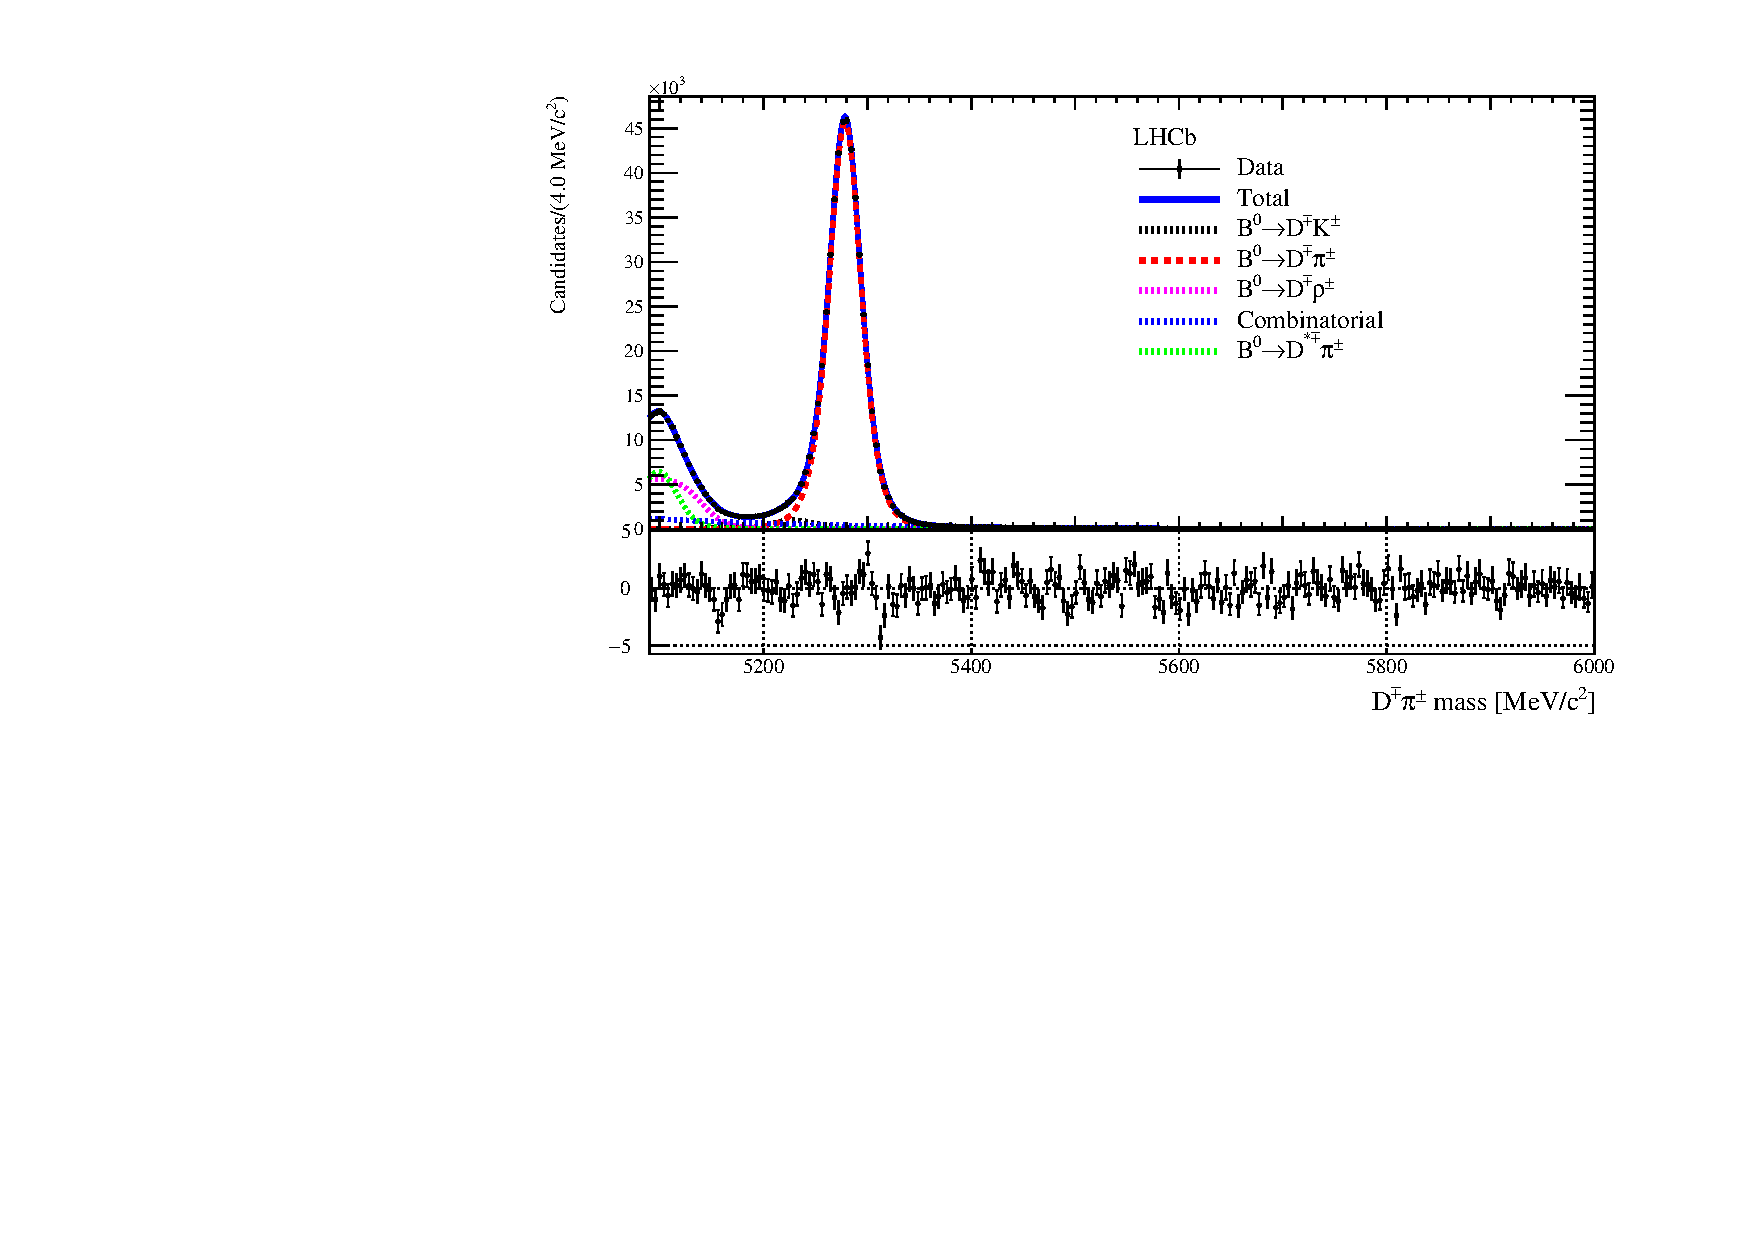
\includegraphics[width=0.75\textwidth]{08MassFit/figs/MDFit_BeautyMass_Bd2DPi_withPulls.pdf}
    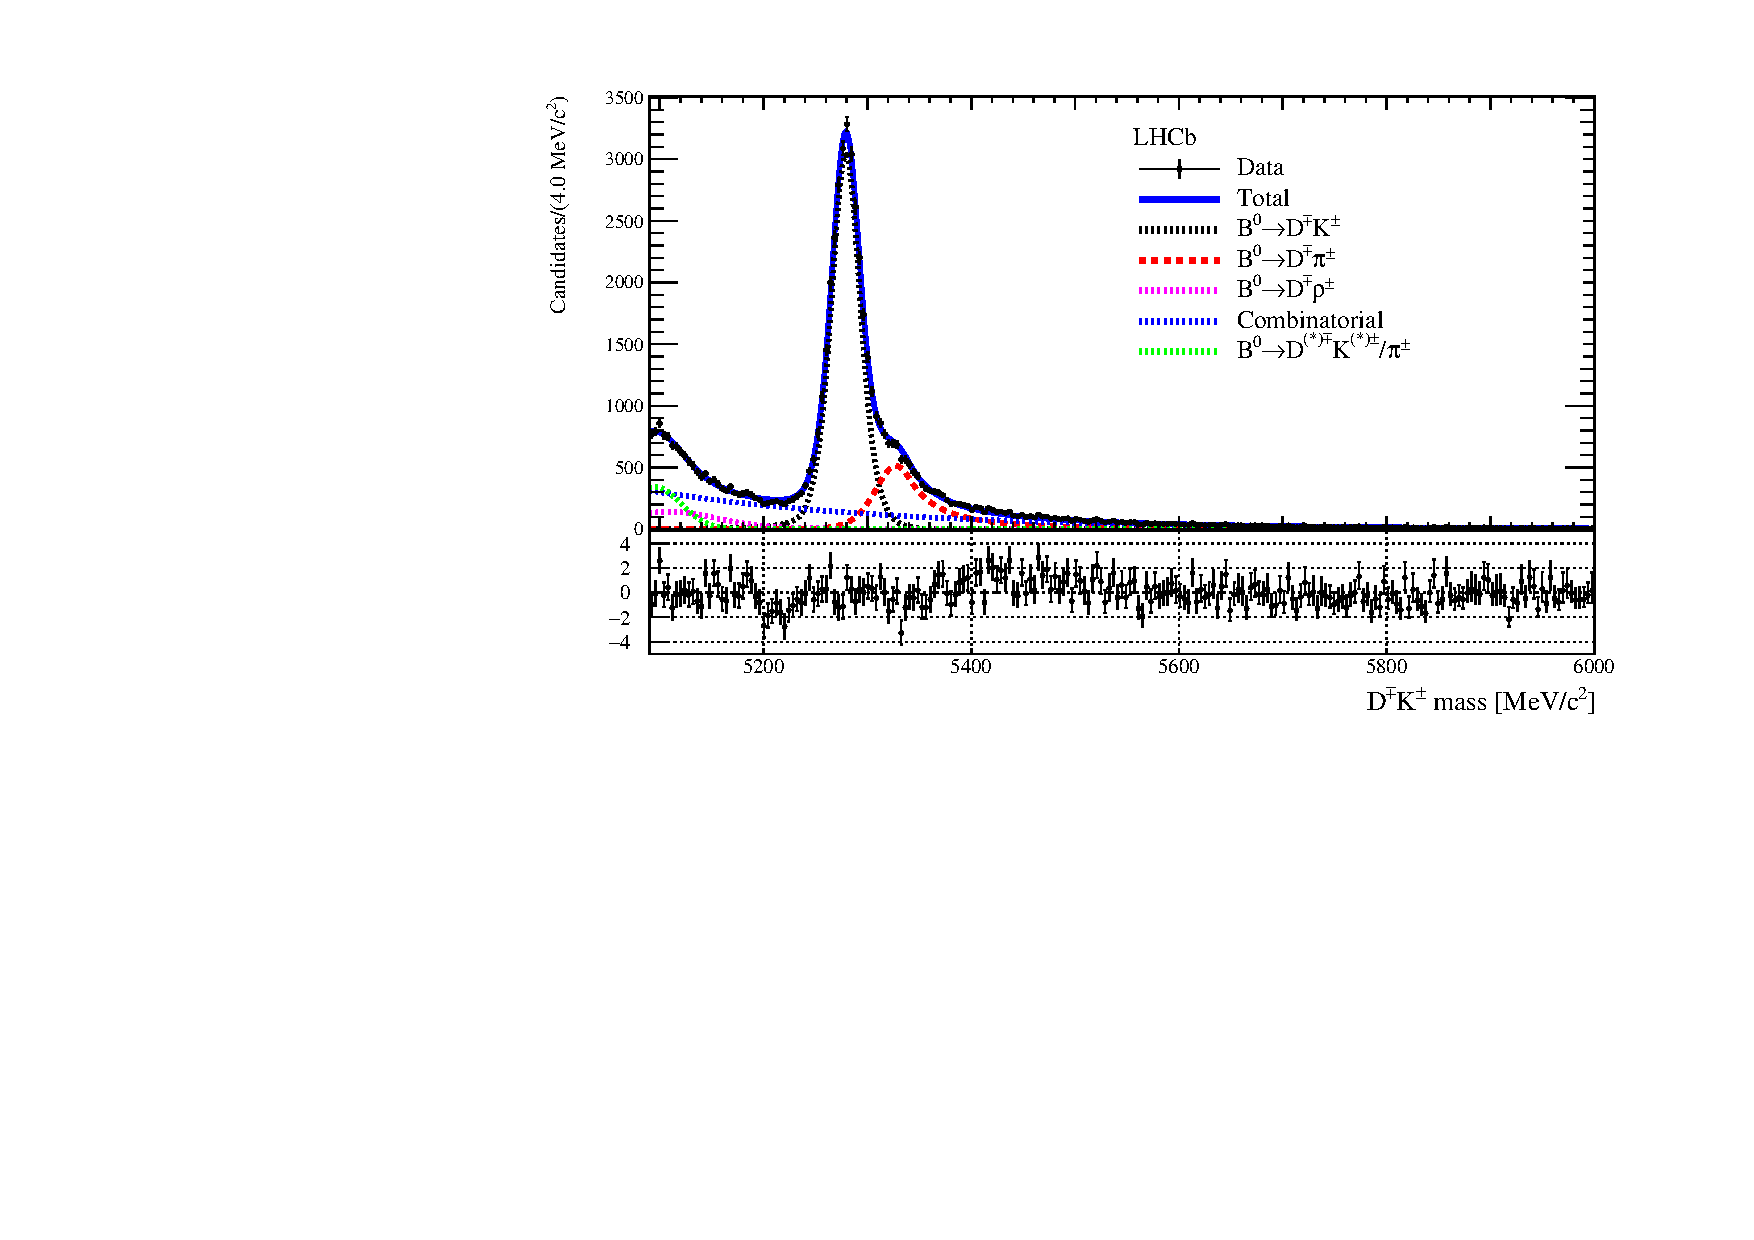
\includegraphics[width=0.75\textwidth]{08MassFit/figs/MDFit_BeautyMass_Bd2DK_withPulls.pdf}
    \caption{Invariant mass distributions of the $\D X$ mass in the \emph{pion} sample (left) and \emph{kaon} sample (right).
    The fit projections of Fit A are overlaid.}
    \label{fig:MassFitPlot}
\end{figure}

After Fit A, an unbinned maximum-likelihood fit to the \emph{pion} sample is performed for which all background components are combined into one single background component and the shapes are fixed to the values found in Fit A.
Futhermore, the fit range is reduced to $[5220, 5600]\,\si[per-mode=symbol]{\MeVcc}$ in order to prevent a dilution of the \emph{sWeights}~\cite{Pivk:2004ty} in later steps of the analysis as all background components, which are neither combinatorial nor close to the signal are removed.
In this second fit (Fit B) only two parameters are floating: the yield $N_{\Bz\!\to\D\pion}^{\pion}$ of the signal \BdToDpi component and a yield $N_{\text{bkg}}^{\pion}$ for the combination of all backgrounds.
These fitted yields are given in \cref{tab:fittedSignalYield}.
\begin{table}[tbp]
	\centering
	\caption{Fitted yields of the signal \BdToDpi component and the combination of all backgrounds in Fit B.}
	\begin{tabular}{cc}
		\toprule
		Parameter & Yield \\
		\midrule
		$N_{\Bz\!\to\D\pion}^{\pion}$	& \num{479045\pm732} \\
		$N_{\text{bkg}}^{\pion}$		& \num{34381\pm300} \\
		\bottomrule
	\end{tabular}
	\label{tab:fittedSignalYield}
\end{table}

As a crosscheck, the full sample is also split by year, polarity and final state and the whole fit procedure is repeated.
The sums of the yields of the corresponding sub samples are then compared to the result given in \cref{tab:fittedSignalYield}.
All comparisons show satisfactory good agreement as shown in \cref{tab:MassFit_Splits}.

\begin{table}[tbp]
	\centering
	\caption{Fitted signal yields in fit B to the pion sample split by year of data taking, magnet polarity and finalstate.
	The last column shows the sum for each split and can be compared with the fitted signal yield in the nominal fit G.}
	\begin{tabular}{SSS}
		\toprule
		{2011} & {2012} & {Sum} \\
		138300\pm400 & 342400\pm600 & 480700\pm700 \\
		\midrule
		{Magnet up} & {Magnet down} & {Sum} \\
		226300\pm500 & 2523\pm500 & 478600\pm700 \\
		\midrule
		{$\Dm\pip$} & {$\Dp\pim$} & {Sum} \\
		242100\pm500 & 237300\pm500 & 479400\pm700 \\
		\bottomrule
	\end{tabular}
	\label{tab:MassFit_Splits}
\end{table}
